\section{2.4 GHz Transceiver SPI Interface}
\label{group__ro__transceiver__spi}\index{2.4 GHz Transceiver SPI Interface@{2.4 GHz Transceiver SPI Interface}}
Routines for accessing the Freescale MC13192 2.4GHz Transceiver.  
\subsection*{Data Structures}
\begin{CompactItemize}
\item 
struct {\bf tx\_\-packet\_\-t}
\item 
struct {\bf rx\_\-packet\_\-t}
\end{CompactItemize}
\subsection*{Defines}
\begin{CompactItemize}
\item 
\#define {\bf TRANSCEIVER\_\-CS}~2
\end{CompactItemize}
\subsection*{Functions}
\begin{CompactItemize}
\item 
void {\bf write\_\-to\_\-spi} (uint8\_\-t spi\_\-adress, uint16\_\-t spi\_\-data)
\item 
void {\bf write\_\-to\_\-ram} (uint8\_\-t spi\_\-adress, {\bf tx\_\-packet\_\-t} $\ast$tx\_\-packet)
\item 
uint8\_\-t {\bf read\_\-from\_\-spi} (uint8\_\-t spi\_\-addr)
\item 
uint8\_\-t {\bf read\_\-from\_\-ram} (uint8\_\-t spi\_\-adress, {\bf rx\_\-packet\_\-t} $\ast$rx\_\-packet)
\end{CompactItemize}


\subsection{Detailed Description}
Routines for accessing the Freescale MC13192 2.4GHz Transceiver. 



\begin{Code}\begin{verbatim} #include <transceiver_spi.h> 
\end{verbatim}\end{Code}



This Routines are for reading and writing to the 802.14.1 Transceiver using the SPI interface

\begin{Desc}
\item[Note:]Based on Atmel Datasheet for Atmega128, Nov. 2006 and on the Freescale reference manual v1.5, 10/2005 for MC13192\end{Desc}
\begin{Desc}
\item[Author:]Rainer Ostendorf \end{Desc}


\subsection{Define Documentation}
\index{ro_transceiver_spi@{ro\_\-transceiver\_\-spi}!TRANSCEIVER_CS@{TRANSCEIVER\_\-CS}}
\index{TRANSCEIVER_CS@{TRANSCEIVER\_\-CS}!ro_transceiver_spi@{ro\_\-transceiver\_\-spi}}
\subsubsection{\setlength{\rightskip}{0pt plus 5cm}\#define TRANSCEIVER\_\-CS~2}\label{group__ro__transceiver__spi_g519ebaa5219cbb279c51e03a48c90f1e}




Definition at line 49 of file transceiver\_\-spi.h.

Referenced by read\_\-from\_\-ram(), read\_\-from\_\-spi(), write\_\-to\_\-ram(), and write\_\-to\_\-spi().

\subsection{Function Documentation}
\index{ro_transceiver_spi@{ro\_\-transceiver\_\-spi}!read_from_ram@{read\_\-from\_\-ram}}
\index{read_from_ram@{read\_\-from\_\-ram}!ro_transceiver_spi@{ro\_\-transceiver\_\-spi}}
\subsubsection{\setlength{\rightskip}{0pt plus 5cm}uint8\_\-t read\_\-from\_\-ram (uint8\_\-t {\em spi\_\-adress}, {\bf rx\_\-packet\_\-t} $\ast$ {\em rx\_\-packet})}\label{group__ro__transceiver__spi_gd0ae0e71ecdd034c8d3d627a28b4325c}




Definition at line 70 of file transceiver\_\-spi.c.

References rx\_\-packet\_\-t::data\-Length, rx\_\-packet\_\-t::datan, spi\_\-cs(), spi\_\-write\_\-16\_\-nocs(), spi\_\-write\_\-8\_\-nocs(), and TRANSCEIVER\_\-CS.

Referenced by get\_\-rx\_\-pkt().

Here is the call graph for this function:\begin{figure}[H]
\begin{center}
\leavevmode
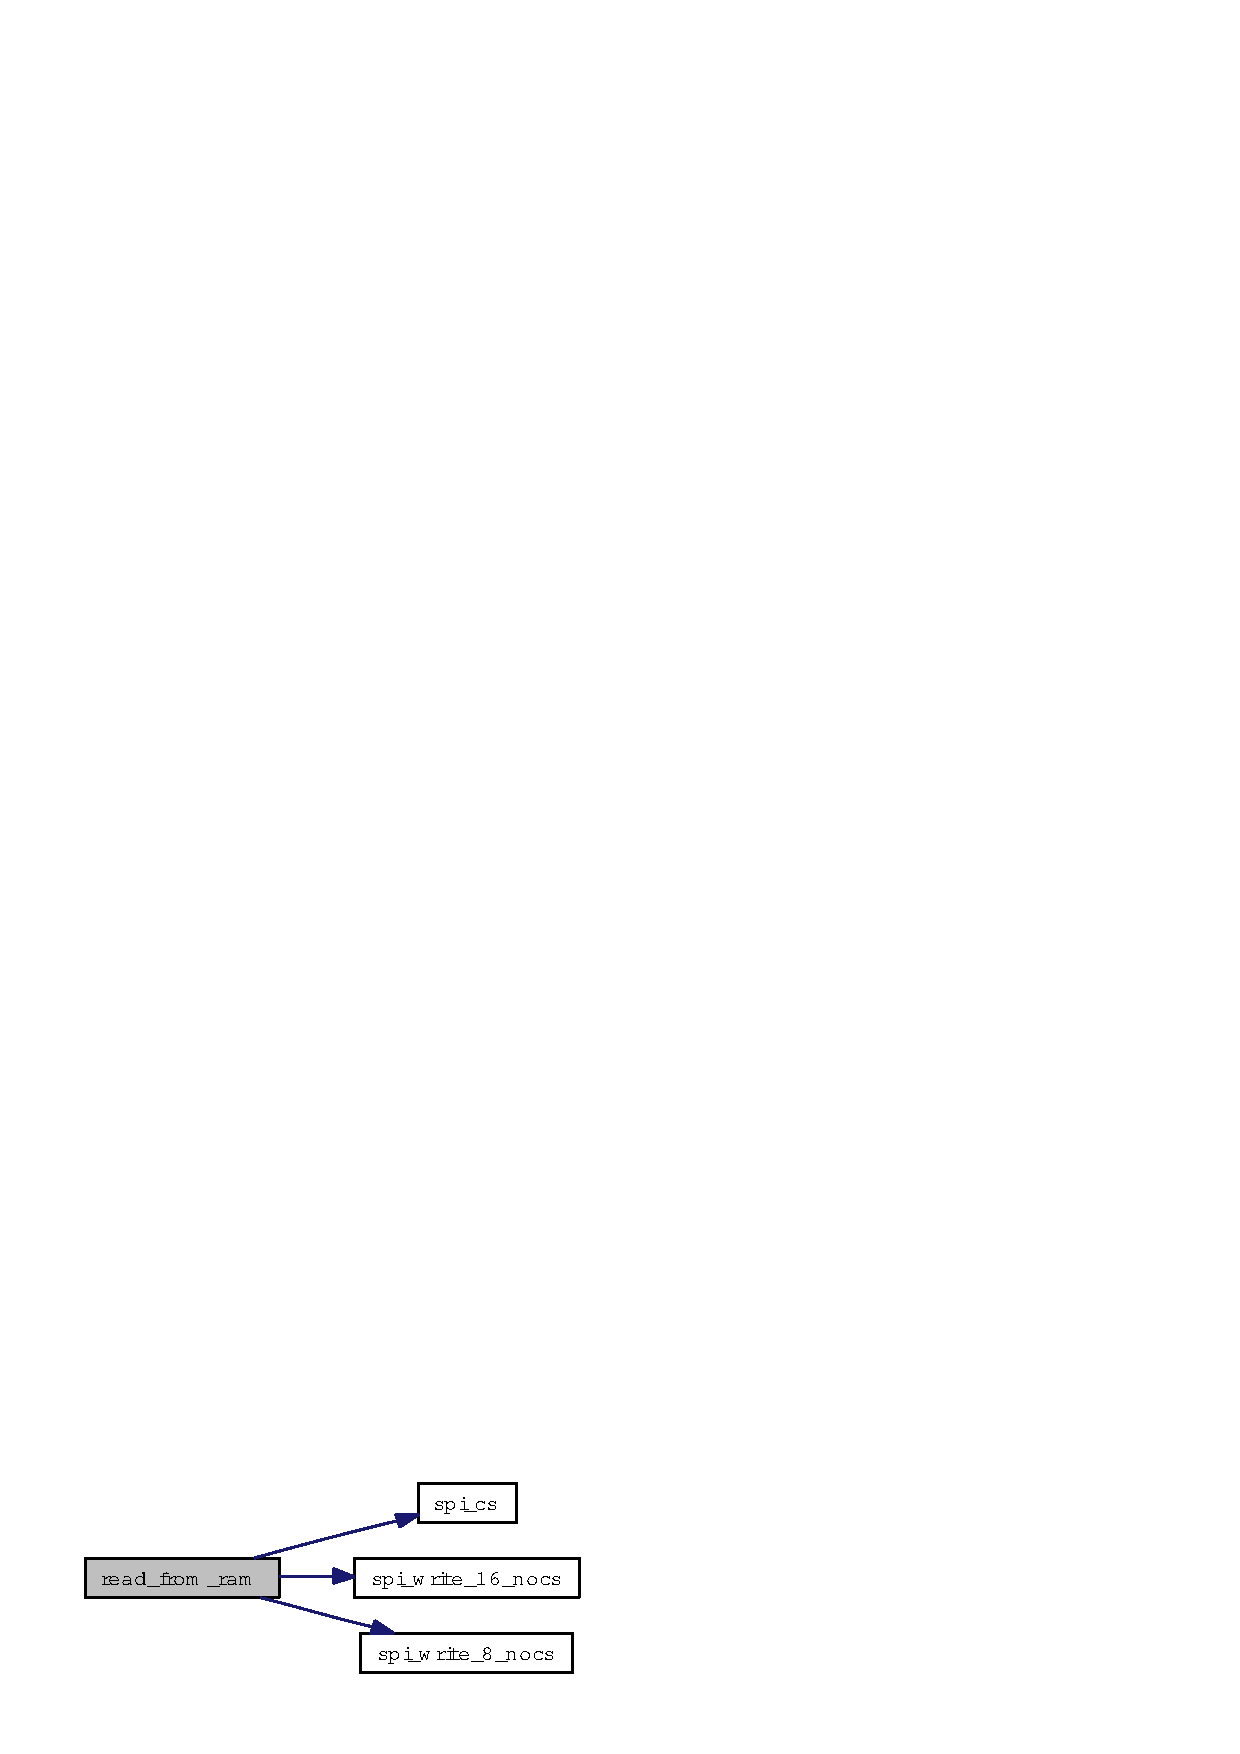
\includegraphics[width=141pt]{group__ro__transceiver__spi_gd0ae0e71ecdd034c8d3d627a28b4325c_cgraph}
\end{center}
\end{figure}
\index{ro_transceiver_spi@{ro\_\-transceiver\_\-spi}!read_from_spi@{read\_\-from\_\-spi}}
\index{read_from_spi@{read\_\-from\_\-spi}!ro_transceiver_spi@{ro\_\-transceiver\_\-spi}}
\subsubsection{\setlength{\rightskip}{0pt plus 5cm}uint8\_\-t read\_\-from\_\-spi (uint8\_\-t {\em spi\_\-addr})}\label{group__ro__transceiver__spi_gb94dfe7c6637b90955520ce14dffbfd2}




Definition at line 41 of file transceiver\_\-spi.c.

References spi\_\-cs(), spi\_\-write\_\-16\_\-nocs(), spi\_\-write\_\-8\_\-nocs(), and TRANSCEIVER\_\-CS.

Referenced by cca\_\-modus(), get\_\-rx\_\-pkt(), MC13192\_\-init(), and MC13192\_\-update\_\-state().

Here is the call graph for this function:\begin{figure}[H]
\begin{center}
\leavevmode
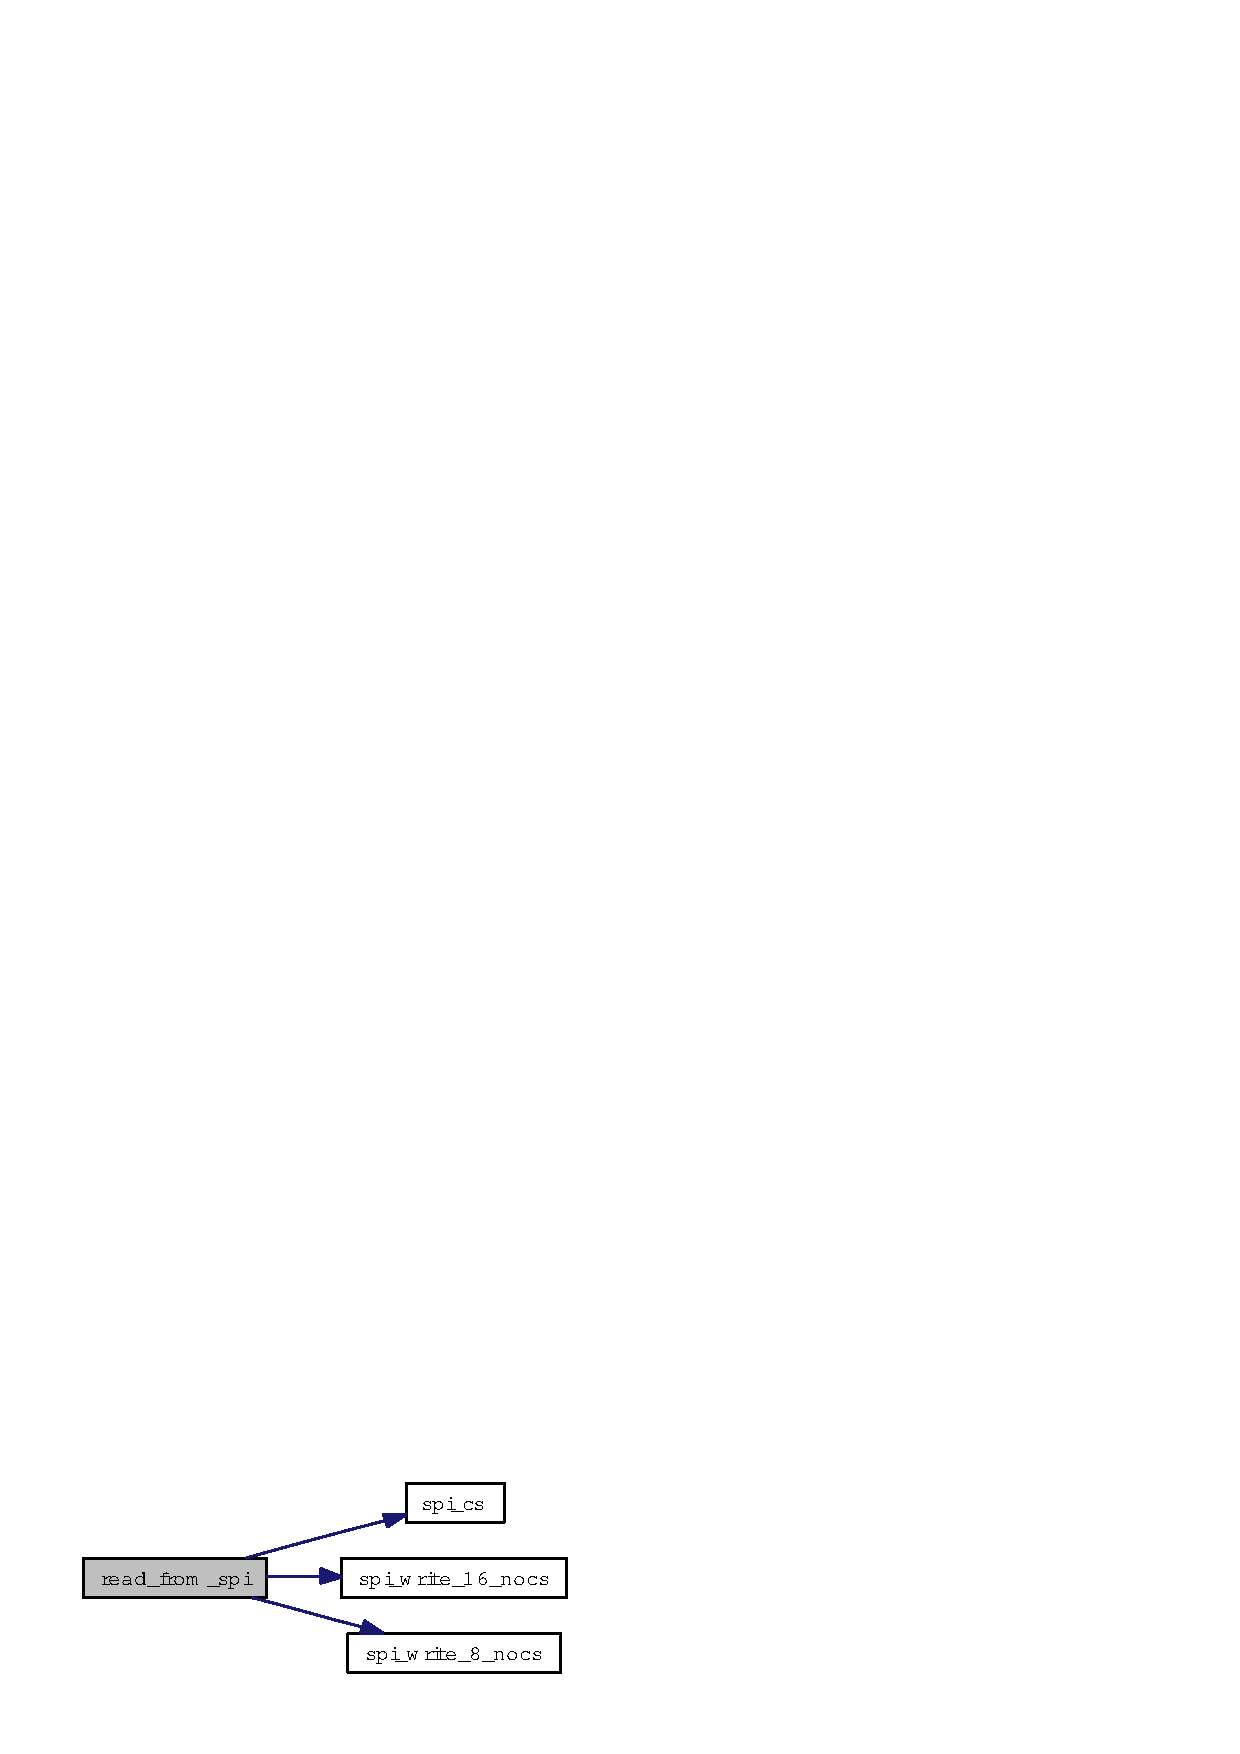
\includegraphics[width=138pt]{group__ro__transceiver__spi_gb94dfe7c6637b90955520ce14dffbfd2_cgraph}
\end{center}
\end{figure}
\index{ro_transceiver_spi@{ro\_\-transceiver\_\-spi}!write_to_ram@{write\_\-to\_\-ram}}
\index{write_to_ram@{write\_\-to\_\-ram}!ro_transceiver_spi@{ro\_\-transceiver\_\-spi}}
\subsubsection{\setlength{\rightskip}{0pt plus 5cm}void write\_\-to\_\-ram (uint8\_\-t {\em spi\_\-adress}, {\bf tx\_\-packet\_\-t} $\ast$ {\em tx\_\-packet})}\label{group__ro__transceiver__spi_g3b940cb98dd035ed3061a30b758adb9c}




Definition at line 53 of file transceiver\_\-spi.c.

References tx\_\-packet\_\-t::data\-Length, tx\_\-packet\_\-t::datan, spi\_\-cs(), spi\_\-write\_\-16\_\-nocs(), spi\_\-write\_\-8\_\-nocs(), and TRANSCEIVER\_\-CS.

Referenced by tx\_\-pkt\_\-mode().

Here is the call graph for this function:\begin{figure}[H]
\begin{center}
\leavevmode
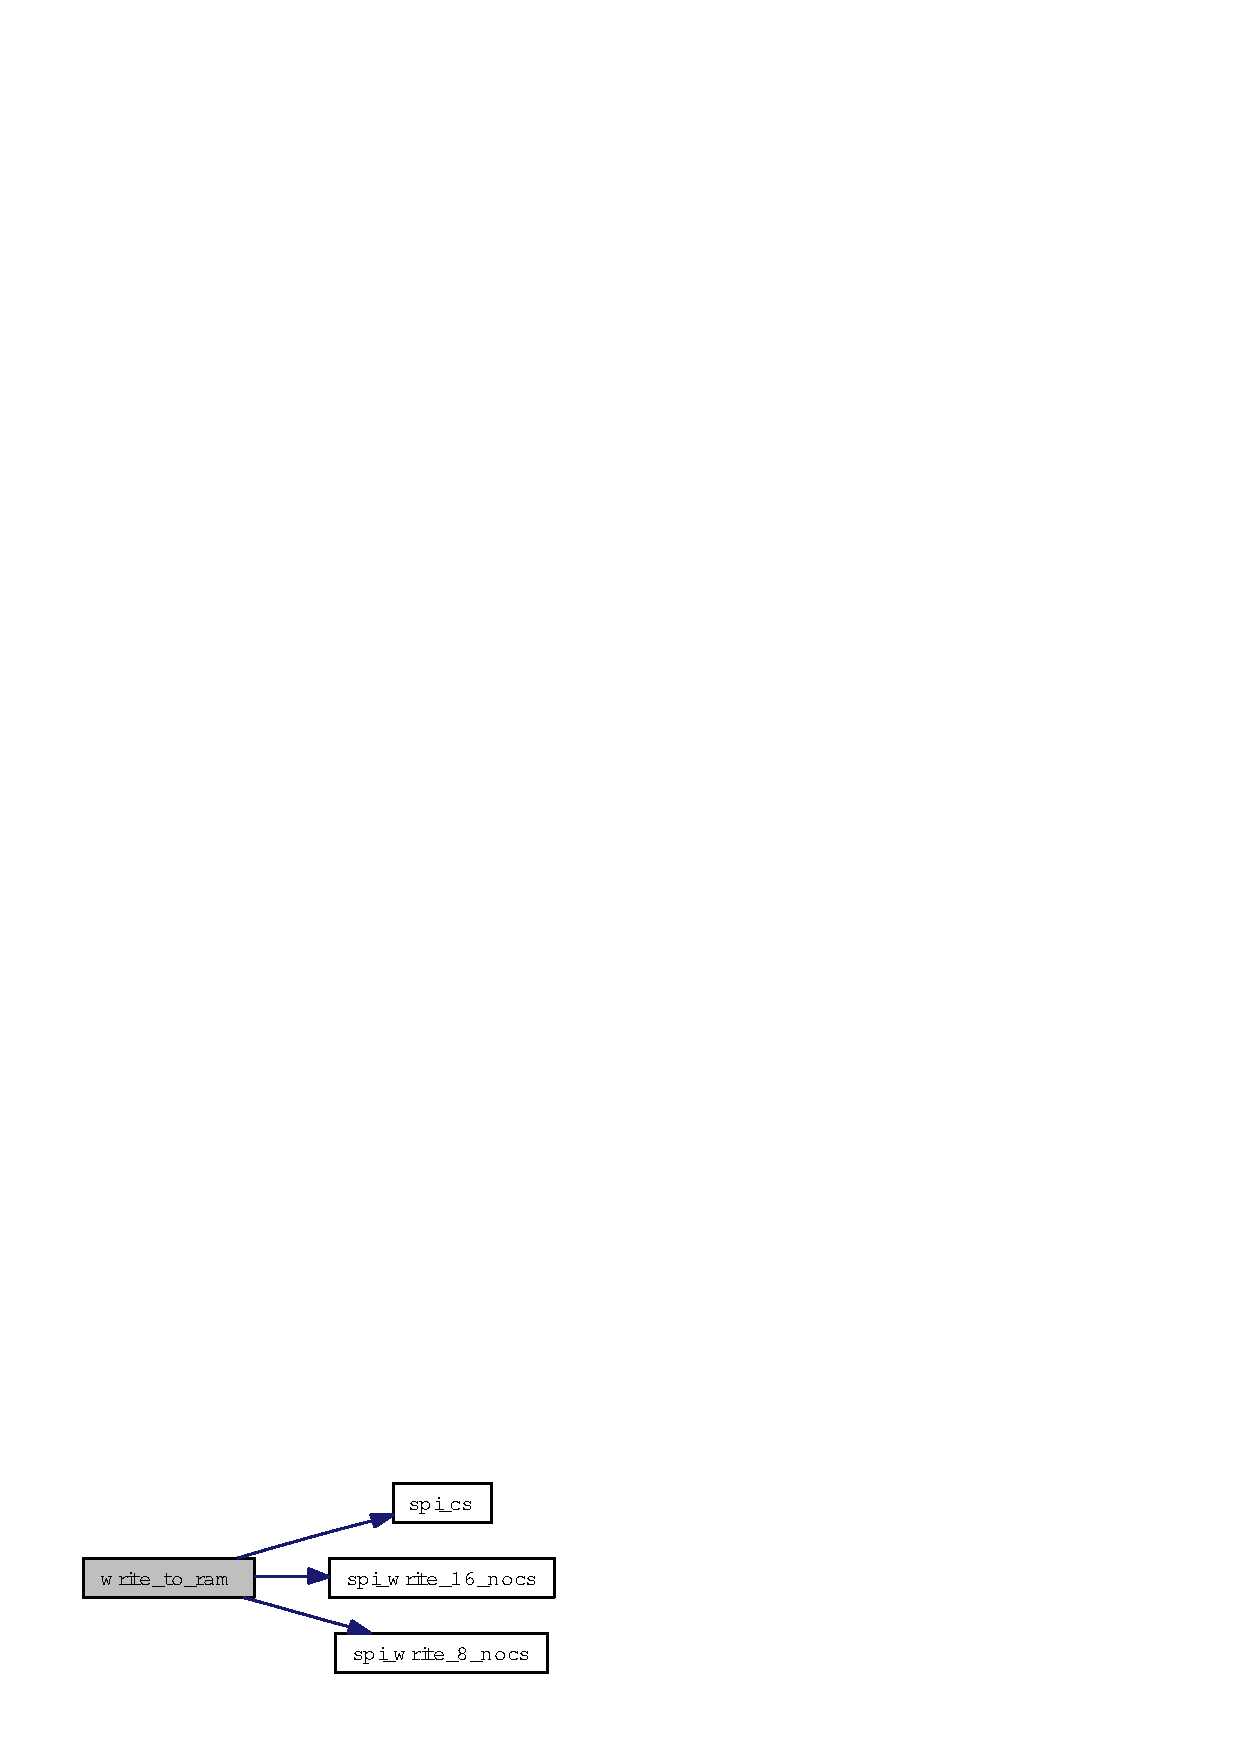
\includegraphics[width=135pt]{group__ro__transceiver__spi_g3b940cb98dd035ed3061a30b758adb9c_cgraph}
\end{center}
\end{figure}
\index{ro_transceiver_spi@{ro\_\-transceiver\_\-spi}!write_to_spi@{write\_\-to\_\-spi}}
\index{write_to_spi@{write\_\-to\_\-spi}!ro_transceiver_spi@{ro\_\-transceiver\_\-spi}}
\subsubsection{\setlength{\rightskip}{0pt plus 5cm}void write\_\-to\_\-spi (uint8\_\-t {\em spi\_\-adress}, uint16\_\-t {\em spi\_\-data})}\label{group__ro__transceiver__spi_gafa419512a4d33e445196d0d63ae6693}




Definition at line 31 of file transceiver\_\-spi.c.

References spi\_\-cs(), spi\_\-write\_\-16\_\-nocs(), spi\_\-write\_\-8\_\-nocs(), and TRANSCEIVER\_\-CS.

Referenced by cca\_\-modus(), init\_\-rx\_\-pkt\_\-mode(), MC13192\_\-init(), and tx\_\-pkt\_\-mode().

Here is the call graph for this function:\begin{figure}[H]
\begin{center}
\leavevmode
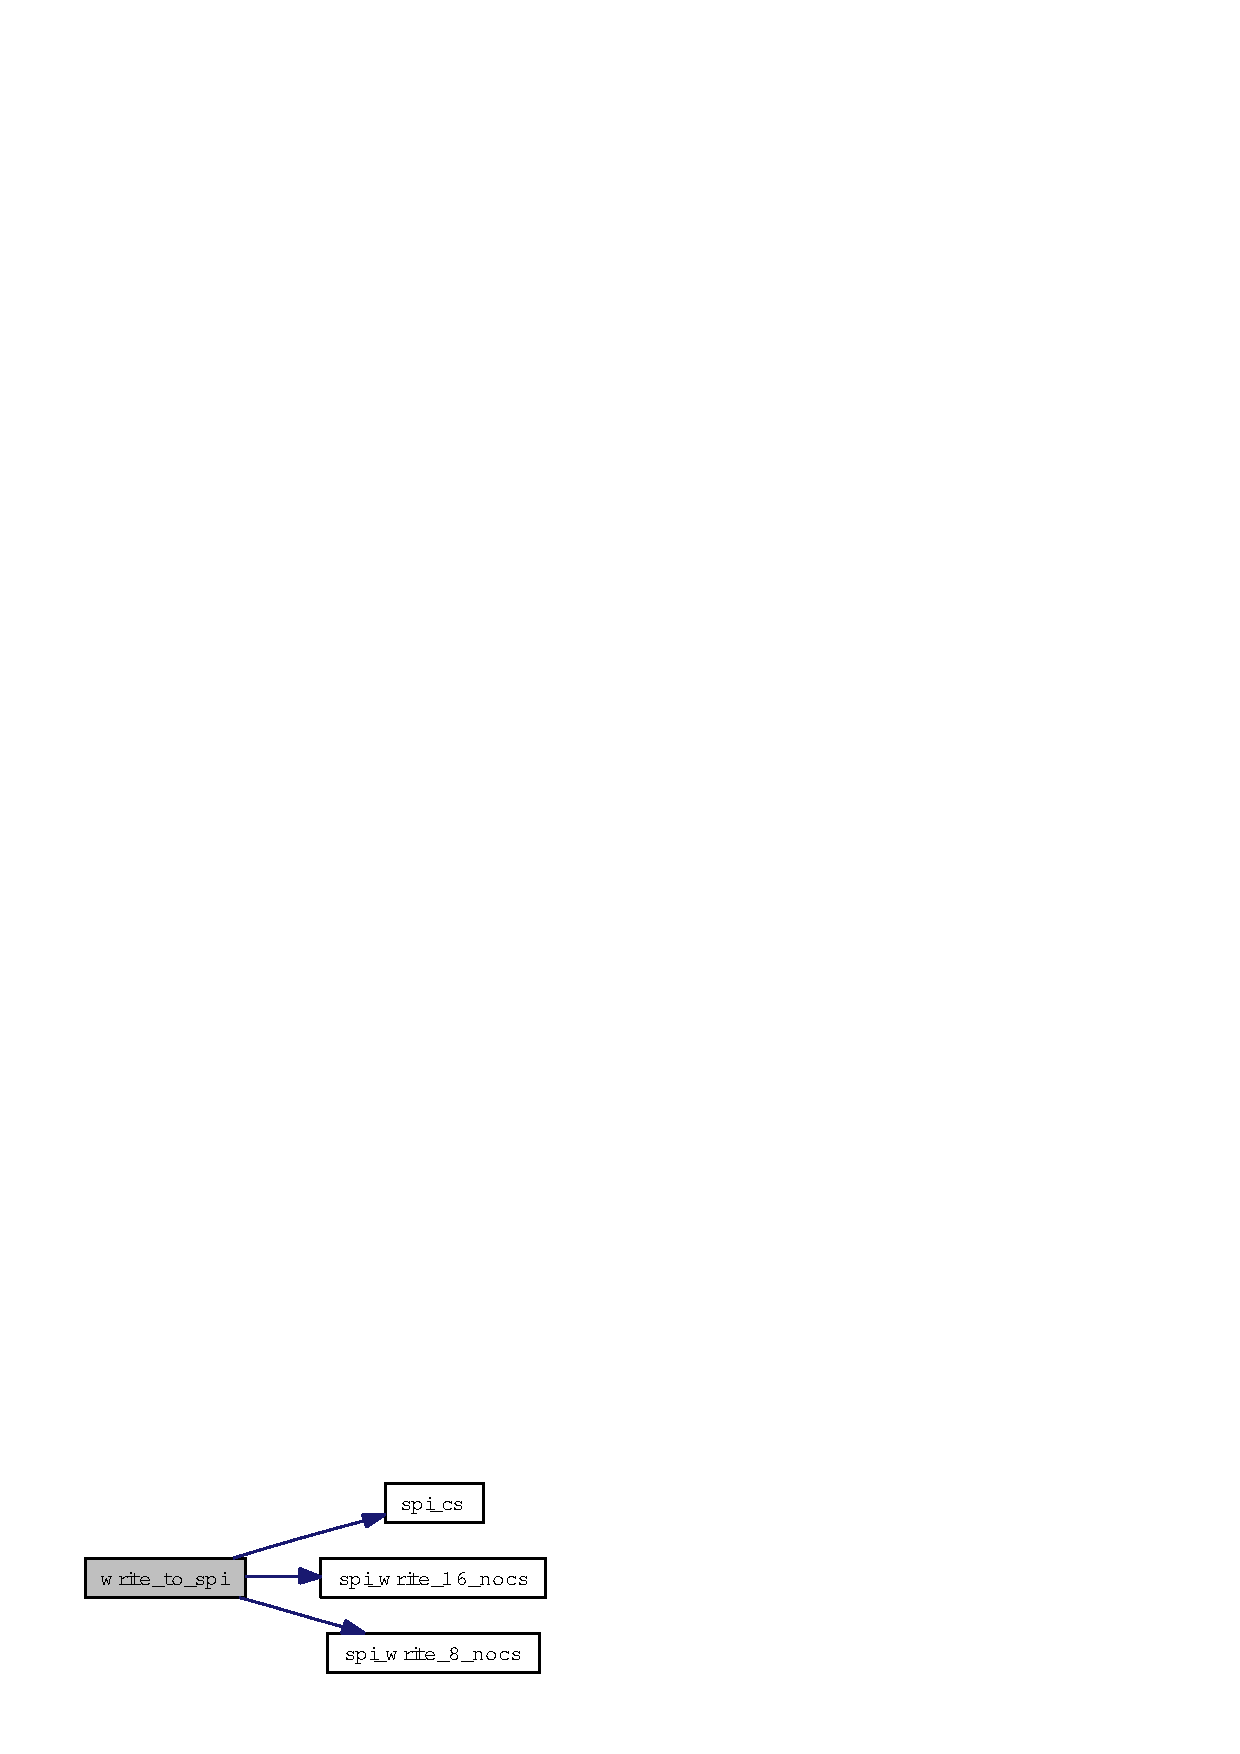
\includegraphics[width=133pt]{group__ro__transceiver__spi_gafa419512a4d33e445196d0d63ae6693_cgraph}
\end{center}
\end{figure}
